% \chapter{Methoden und Praktiken}

%\textit{In diesem Kapitel soll beschrieben werden, wie eine Nachvollziehbarkeit in Webapplikationen erreicht werden kann. Spezielle Methoden und Praktiken sollen vorgestellt und beleuchtet werden.}
% \textit{Hier könnte unter anderem \textbf{OpenTelemetry} betrachtet werden.}

\vspace{-\baselineskip}

\section{Methoden}

\subsection{Logging}

%\textit{Folgende Fragen sollen zur Methode beantwortet werden}
%\begin{enumerate}
%	\item \textit{Gibt es Besonderheiten zu Logging in anderen Projekten (Backend vs. Frontend)?}
%	\item \textit{Wie können Logs an einen auswertenden Stakeholder gelangen?}
%	\item \textit{Welches Verhalten kann hiermit aufgedeckt/nachvollziehbar gemacht werden?}
%\end{enumerate}

Mit Logging bezeichnet man die systematische Protokollierung von Softwareprozessen und ihren internen Zuständen. Mithilfe von Logs, also Protokollen, kann Betreibern und Entwicklern ermöglicht werden, dass sie das Anwendungsverhalten nachvollziehen können. Beispielsweise ist es sinnvoll einen fehlgeschlagenen Login eines Nutzers zu loggen, dabei ist es hilfreich, wenn viele Kontextinformationen mitgeloggt werden. % Nah verwandt mit oder basierend auf Logging sind die Teilgebiete Auditing, Monitoring, Tracing und Operations-Monitoring.

Logging bei Webfrontends stellt eine besondere Hürde dar, denn wie bereits in \autoref{sec:logdaten} geschildert, müssen die Logs an ein Partnersystem weitergeleitet werden.

\subsubsection{Structured Logging}

%\subsection{Monitoring}
%
%\textit{Folgende Fragen sollen zur Methode beantwortet werden}
%\begin{enumerate}
%	\item \textit{Welche Anwendungseigenschaften sind zu monitoren?}
%	\item \textit{Welches Verhalten kann hiermit aufgedeckt/nachvollziehbar gemacht werden?}
%\end{enumerate}

Logmeldungen erfolgen meist textbasiert und in einem menschenlesbaren Format. Wenn nun jedoch Informationen aus einer großen Menge von Logs extrahiert werden sollen, ist so ein simples Format hinderlich. Hierbei kommt Structured Logging ins Spiel, bei dem zwar auch menschenlesbare Logmeldungen produziert werden, aber das Format ist fest definiert und erlaubt einer anderen Software Informationen einfacher zu extrahieren.

\subsection{Metriken}

Mit Metriken versucht man Softwareeigenschaften in Zahlenwerten abzubilden. Diese Zahlenwerte werden über Messungen ermittelt. Beispiele für Metriken sind:

\begin{enumerate}
	\item Eine Zeitmessung, bzgl. der Dauer einer HTTP-Anfrage
	\item Eine Messung der CPU-Auslastung
\end{enumerate}

\nomenclature[Fachbegriff]{HTTP}{Hyper-Text-Transfer-Protocol}
\nomenclature[Fachbegriff]{CPU}{Central Processing Unit, auf Deutsch \enquote{Prozessor}.} 

Mit den Ergebnissen lassen sich wiederum Rückschlüsse zur Softwareeigenschaft ziehen, dass bspw. eine Anfrage deutlich länger benötigt als andere \enquote{gleichwertige} Anfragen. Weiterhin lassen sich historische Veränderungen in den Metriken erkennen und können unerwünschte Abweichungen aufdecken.

\subsection{Tracing}
\label{sec:tracing}

Tracing beschäftigt sich mit dem Aufzeichnen von Kommunikationsflüssen. Hierbei erfasst Tracing einerseits die Kommunikationsflüsse innerhalb einer Applikation oder innerhalb eines Systems. Andererseits zeichnet Tracing aber auch die Kommunikationsflüsse bei verteilten Systemen auf, um diese, meist komplexen Zusammenhänge, zu veranschaulichen. Ein herstellerunabhängiger Standard, der sich aus diesem Gebiet entwickelt hat, ist OpenTracing \cite{OpenTracing}.

OpenTracing definiert zwei grundlegende Objekte: Traces und Spans. Ein Trace ist eine Menge an Events, die über eine einzelne logische Aktion - wie z. B. den Druck eines Knopfes - ausgelöst wurde oder resultiert. Spans besitzen den Namen einer Methode oder Operation, welche der Span umschließt. Wird in der Methode oder Operation eine weitere Methode oder Operation aufgerufen, welche von einem Span umschlossen ist, so ist dies nun ein Kindspan des ursprünglichen Spans. Spans haben einen Start- sowie einen Endzeitpunkt und sie speichern die Beziehung zu ihrem Elternspan (außer es handelt sich um den \enquote{root}-Span). Sie können darüber hinaus Attribute enthalten, sowie eingetretene Events.

OpenTracing definiert Traces implizit über ihre Spans. Ein Trace ist damit ein gerichteter Graph ohne Zyklus, wobei die Knoten hierbei die Spans darstellen und die Kanten die Eltern-/Kindbeziehung veranschaulichen \cite{OpenTracingSpecification}. Ein beispielhafter Trace mit seinen Spans und deren Beziehungen ist in \autoref{fig:otel-causal-relationship} zu betrachten. Die zeitliche Reihenfolge der Spans kann auch eine hilfreiche Visualisierung sein, um die Entwicklung der Spans zu verstehen \citationneeded (vgl. \autoref{fig:otel-temporal-relationship}). Diese Definition wurde in den Nachfolgestandard OpenTelemetry aufgenommen und an späterer Stelle erläutert.

Ein verteilter Trace, oftmals \enquote{Distributed Trace} genannt, ist ein Trace, der sich aus den Events von verschiedenen Systemen zusammensetzt, die miteinander kommunizieren. Hierbei beinhaltet der Trace Events, die über die Grenzen von Anwendungen, Prozessen und Netzwerken hinaus gehen \cite{OpenTracingSpecification}.

\begin{minipage}{.47\textwidth}
	\centering
	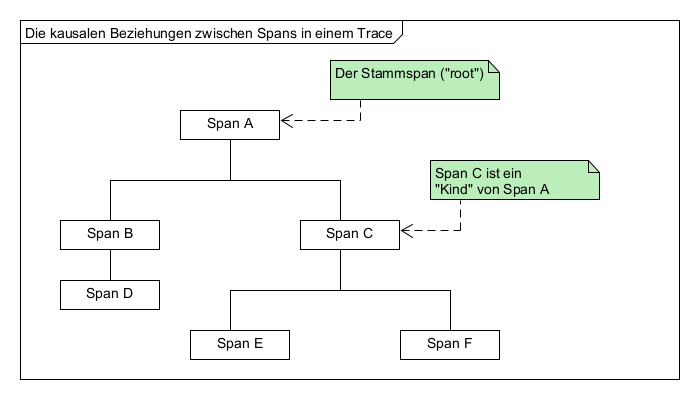
\includegraphics[width=\linewidth]{img/03_methoden/otel_causal-relationship.png}
	\captionof{figure}{Kausale Beziehung zwischen Spans. Eigene Darstellung.}
	\label{fig:otel-causal-relationship}
\end{minipage}%
\hspace{.06\textwidth}
\begin{minipage}{.47\textwidth}
	\centering
	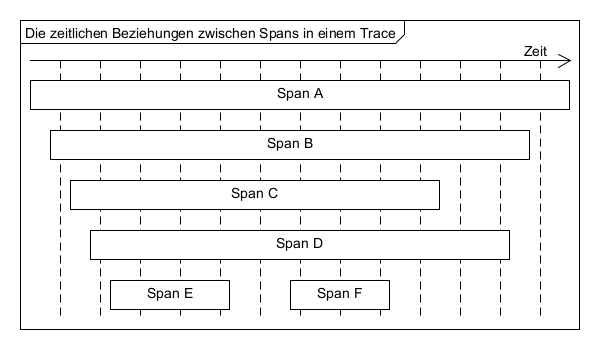
\includegraphics[width=\linewidth]{img/03_methoden/otel_temporal-relationship}
	\captionof{figure}{Zeitliche Beziehung zwischen Spans. Eigene Darstellung.}
	\label{fig:otel-temporal-relationship}
\end{minipage}

\subsection{Fehlerberichte}

\begin{wrapfigure}[15]{r}{0.4\textwidth}
\centering
\vspace{-\baselineskip}
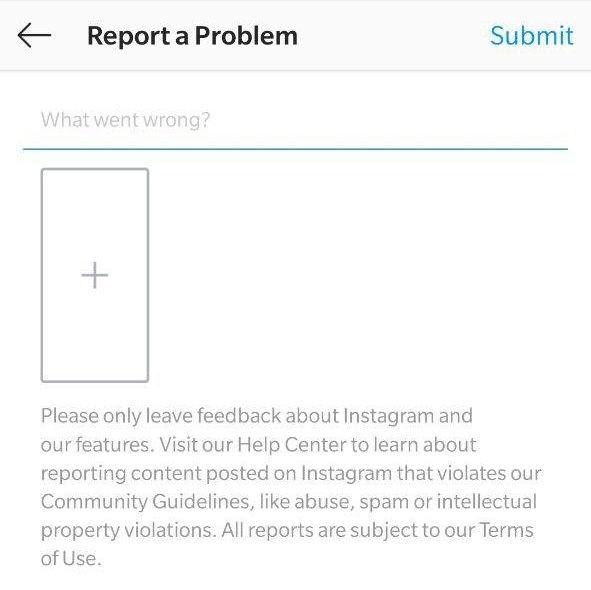
\includegraphics[width=\linewidth]{img/instagram-feedback/instagram-feedback.jpg}
\caption{Fehlerbericht in der Instagram App \cite{Instagram}}
\label{fig:instagram-bug-report}
\end{wrapfigure}

Fehlerberichte sind ein klassisches Mittel, um den Nutzer selber aktiv werden zu lassen und zu erfragen, welche Aktionen er durchgeführt hat und was schiefgelaufen ist (vgl \autoref{fig:instagram-bug-report}). Hiermit können Fehler, aber auch unverständliche Workflows, aufgedeckt werden. Weiterhin kann die Intention des Nutzers ermittelt werden, vorausgesetzt er gibt dies an.

Bettenburg \etal \cite{WhatMakesAGoodBugReport} fanden jedoch Mängel bei der Effektivität von Fehlerberichten. Denn Nutzer meldeten Informationen und Details, die sich für die Entwickler als nicht allzu hilfreich herausstellten. Diese Diskrepanz kann u. A. dadurch erläutert werden, dass Nutzer im Regelfall kein technisches Verständnis vom System vorweisen.

Hinzukommend muss man beachten, dass die User Experience negativ beeinflusst werden kann, wenn ein Nutzer einen Dialog mit einem Aufruf für einen Fehlerbericht erhält - gerade wenn der Fehler ihn selbst nicht eingeschränkt hat.

\section{Praktiken aus der Wirtschaft}

In der Fachpraxis haben sich einige Technologien über die Jahre entwickelt und etabliert, die eine verbesserte Nachvollziehbarkeit als Ziel haben. Neben den zuvor vorgestellten Methoden haben sich bei Technologien einige Praktiken entwickelt, die teilweise auf den Methoden aufbauen oder neue Konzepte darstellen, um ihr Ziel zu erreichen. Diese Praktiken werden folgend vorgestellt.

\subsection{Observability}

Observability ist der Oberbegriff, der sich in der Wirtschaft entwickelt hat, um Werkzeuge zu beschreiben, die eine bessere Nachvollziehbarkeit versprechen. Es kann mit \enquote{Beobachtbarkeit} übersetzt werden, aber ließe sich auch freier mit Nachvollziehbarkeit gleichsetzen. Observability enstand aus dem klassischen Monitoring von Software, aber beinhaltet neben Monitoring noch einige weitere Disziplinen, wie Logging, Tracing und Metriken. Graf \cite{MichaelGrafBA} definiert Observability wie folgt:

%Observability hat allgemeiner als Ziel, dass Anwendungen und Systeme exakt betrachtet werden können, um den Verantwortlichen zu ermöglichen, dass  \cite{DistributedSystemsObservability}.

\begin{quotation}
Ziel ist es, Anwendungen und Systeme exakt zu beobachten, Informationen über technische Fehlfunktionen zu erhalten und schnell an die Verantwortlichen zu übermitteln. Logfiles, Informationen zur Ressourcennutzung und Anwendungs-Traces sollen den Administratoren und Entwicklern dabei helfen, die Fehlerursachen zu erkennen, die Probleme zu beheben und künftige Ausfälle nach Möglichkeit zu vermeiden \cite{DistributedSystemsObservability}.
\end{quotation}

\subsection{System Monitoring}

System Monitoring beschäftigt sich mit der Überwachung der notwendigen Systeme und Dienste in Bezug auf Hardware- und Softwareressourcen. Es handelt sich hierbei um ein projektunabhängiges Monitoring, welches sicherstellen soll, dass die Infrastruktur funktionstüchtig bleibt.

Ein Beispiel für System Monitoring wäre u. A., wenn man ein Menge an Systemen auf die Festplatten- und CPU-Auslastung hin kontrolliert und überwacht. Es können weitere Aspekte überwacht werden, aber im Regelfall hat die Überwachung selbst nichts mit einem eigentlichen Projekt zu tun, außer dass die Infrastruktur hierfür sichergestellt wird.

\subsection{Log Management}

Log Management umfasst die Erfassung, Speicherung, Verarbeitung und Analyse von Logdaten von Anwendungen. Weiterhin bieten Werkzeuge hierbei oftmals fundierte Such- und Meldefunktionen. Um die Daten aus einer Anwendung heraus zu exportieren, werden oftmals eine Vielzahl an Integrationen für Frameworks und Logbibliotheken angeboten.

Einer der wichtigsten Punkte im Log Management, ist der Umgang mit großen Datenmengen und die gewünschten Operationen, die Nutzer damit durchführen möchten.

\subsection{Application Performance Monitoring (APM)}

Beim Application Performance Monitoring werden Daten innerhalb von Applikationen gesammelt, die Rückschlüsse auf die Performanz von bspw. Transaktionen geben sollen \cite{StudyingTheEffectivenessOfAPMTools}. Mit diesen Daten können dann Regressionen der Performanz, in Aspekten wie Zeitaufwand oder Ressourcennutzung, festgestellt werden.

Neben allgemeinen Aspekten, die sich auf den Prozess- oder Ausführungskontext beziehen, können aber auch spezifische Faktoren, wie die Ausführungszeit einer wichtigen Methode, veranschaulicht werden. APM wird zum Großteil mit Metriken realisiert, welche die zu untersuchenden Aspekte in numerischen Werten wiedergeben.

\subsection{Real User Monitoring (RUM)}

Real User Monitoring beschäftigt sich mit dem Mitschneiden von allen Nutzerinteraktionen mit bspw. einer Webapplikation. Hiermit lässt sich nachvollziehen, wie ein Nutzer die Anwendung verwendet. RUM kann dazu verwendet werden um Herauszufinden, wie ein Nutzer zu einem Zustand gelangt ist. Aber es können auch ineffiziente Klickpfade hierdurch festgestellt werden und darauf basierend UX Verbesserungen vorgenommen werden.

Häufig wird RUM aber nicht verwendet, um einzelne Nutzerinteraktionen nachvollziehbar zu machen, sondern es werden oft gruppierte Verhaltensweisen erfasst, um allgemeine Schlüsse über eine Anwendung ziehen zu können.

\subsection{Synthetic Monitoring}

Beim Synthetic Monitoring werden Endnutzerszenarien simuliert, um zu prüfen und sicherzustellen, dass diese Szenarien wie gewünscht ablaufen. Hierbei kann auf Aspekte wie Funktionalität, Verfügbarkeit und auch verstrichene Zeit kontrolliert werden.

\subsection{Error/Crash Monitoring}

Das Error Monitoring konzentriert sich auf das Erfassen und Melden von Fehlern. Es werden oftmals neben dem eigentlichen Fehler auch Aspekte vom RUM und Logging gemeldet, um mehr Kontextinformationen zu liefern.

Das Error Monitoring wird oftmals eng mit einem Issue-Management verbunden, da aufgetretene Fehler meist zu einem Issue werden oder werden sollten und eine Nachverfolgbarkeit der Fehlerbehebung hierbei Sinn macht.

\subsection{Session-Replay}

Session-Replay bedeutet, dass eine Sitzung eines Nutzers nachgestellt wird, so als ob sie gerade passiert. Hierbei können einzelne Aspekte der Anwendung nachgestellt werden, bspw. der Kommunikationsablauf, bei dem die tatsächliche zeitliche Abfolge von Kommunikationen nachvollzogen werden können. Desto mehr Aspekte nachgestellt werden, desto realitätsnaher ist die Simulation und entsprechend hilfreich ist sie beim Nachvollziehen.

Session-Replay nimmt so eine enorme Datenmenge für jede Nutzersitzung auf und benötigt so ein gutes Konzept im Datenmangement, aber besonders bei Browsern wird eine effiziente Kommunikation benötigt.

\newpage

\section{Werkzeuge und Technologien}
\label{sec:werkzeuge-und-technologien}

%\textit{Basierend auf dem Grundwissen über die Methoden und Praktiken, soll nun der Stand der Technik erörtert werden. Hierbei sollen Werkzeuge und Technologien und ihre Ansätze hervorgehoben werden und mit Hilfe welcher Methoden sie welches Ziel erreichen.}
%
%\textit{Wie in der Zielsetzung definiert sollen hier zwei bis drei Technologien näher vorgestellt werden.}
%
%\textit{Weiterhin könnte beleuchtet werden, wie ähnliche Herausforderungen bei anderen „Fat-Client“-Lösungen (also nicht SPAs) angegangen werden, und kann man hier vielleicht etwas lernen oder übertragen (und wenn nicht, warum nicht)?}

\subsection{Fachpraxis}

Bei der Recherche zu Werkzeugen und Technologien aus der Fachpraxis wurden einige Produkte näher betrachtet. Folgend werden die Ergebnisse beschrieben, welche aber nicht als Vergleich oder Produktbeschreibung dienen, sondern eher, um ein grobes Verständnis der Fachpraxis zu vermitteln, um im Verlauf der Arbeit darauf zurückgreifen zu können. Bei der Recherche kam wiederholt der Begriff OpenTelemetry auf, deswegen und aufgrund der Beziehung zu OpenTracing wird der Standard folgend kurz beschrieben.

\subsubsection{OpenTelemetry}

\begin{wrapfigure}[19]{r}{0.35\textwidth}
\centering
\vspace{-3\baselineskip}
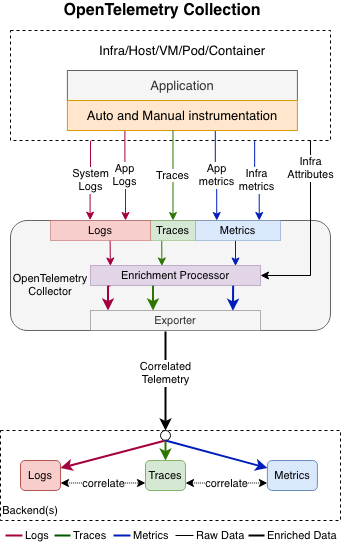
\includegraphics[width=\linewidth]{img/03_methoden/otel_unified-collection_2.png}
\caption{Schaubild einer Lösung auf Basis von OTel \cite{OpenTelemetryUnifiedCollection}}
\label{fig:otel-unified-collection}
\end{wrapfigure}

OpenTelemetry (OTel) \cite{OpenTelemetry} ist ein sich derzeit entwickelnder herstellerunabhängiger Standard, um Tracing-, Metrik- und Logdaten\footnotemark zu erfassen, verarbeiten, analysieren und zu visualisieren. Der Standard fasst die beiden Standards OpenTracing und OpenCensus \cite{OpenCensus} zusammen und hat sich als Ziel gesetzt diese zu erweitern \cite{UseNixDistributiveTracing}. Hinter dem Standard stehen u. A. die Cloud Native Computing Foundation (CNCF), Google, Microsoft, und führende Hersteller von Tracing- und Monitoring-Lösungen. Ein erster Release ist für Ende 2020/Anfang 2021 geplant. Ziel ist es, dass Entwicklertools und -werkzeuge benutzen können, ohne jedesmal eine hochspezifische Anbindung schreiben und konfigurieren zu müssen. Stattdessen definiert der Standard Komponenten, die spezielle Aufgabengebiete haben und mit einer allgemeinen API anzusprechen sind. Die technische Infrastruktur einer auf OTel basierenden Lösung ist in \autoref{fig:otel-unified-collection} zu betrachten. Im groben definiert OTel folgende Komponenten: API, SDK, Exporter, Collector und Backend (vgl. \autoref{fig:otel-components}).

\nomenclature[Fachbegriff]{OTel}{OpenTelemetry}
\nomenclature[Fachbegriff]{CNCF}{Cloud Native Computing Foundation}
\footnotetext{Logging ist noch nicht gut im OTel Standard definiert/aufgenommen \cite{OpenTelemetryLoggingSpecification}}

\begin{figure}[H]
	\centering
	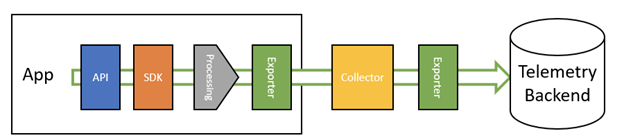
\includegraphics[width=0.55\linewidth]{img/03_methoden/dynatrace_otel-components.png}
	\caption{OTel Komponenten \cite{DynatraceOTelComponents}}
	\label{fig:otel-components}
\end{figure}

\subsubsection{New Relic}

New Relic \cite{NewRelic} ist ein SaaS der gleichnamigen Firma, welcher Betreiber von Softwareprojekten dabei unterstützt das Verhalten ihrer Anwendungen zu überwachen. Der Dienst konzentriert sich auf System Monitoring, APM und RUM und erfasst die notwendigen Daten mit proprietären Lösungen. Neben den Kernfunktionalitäten unterstützt New Relic auch Log Management, Synthetic Monitoring, Tracing und Error Monitoring.

\nomenclature[Fachbegriff]{SaaS}{Software-as-a-Service}

Bei New Relic wurde die kostenlose Version aufgesetzt und evaluiert. Der New Relic Agent, welcher die Daten beim Client sammelt, wird über ein Skript eingebunden und sendet in regelmäßigen Abständen Daten an New Relic. Über die Oberfläche von New Relic können dann allgemeine Charakteristika der Clients betrachtet werden, wie Ladezeiten, Browserhersteller, Ajax-Antwortzeiten. Spezielle Eigenschaften eines einzelnen sind jedoch nicht möglich, wahrscheinlich u. A. aus Aspekten des Datenschutzes. Jedoch im Fehlerfall gibt es mehr Informationen, denn hier werden spezifische Daten (Stacktrace, genaue Browserversion, Uhrzeit, ...) zum Fehler sowie zum Client erhoben und in der Oberfläche dargestellt. Diese Informationen sind gut zum Nachvollziehen, dass ein Fehler aufgetreten ist und was die Rahmenbedingungen sind - jedoch sind die Informationen nicht ausreichend, um ein klares Bild des Fehlers zu erhalten. Dies könnte mit dem Log-Management von New Relic komplementiert werden, jedoch wären diese selber zu erheben und an einen eigenen Server zu senden, um dann die Logs an New Relic weiterzuleiten. Des Weiteren wird der Agent standardmäßig von AdBlockern blockiert, sowie von der \enquote{Enhanced Tracking Protection} im Mozilla Firefox. Es ist nicht möglich New Relics Dienst selber zu hosten, es ist also eine sog. \enquote{OnPremise}-Lösung nicht möglich. Des Weiteren wird auch eine Weiterleitung über einen eigens bereitgestellten Proxy nicht unterstützt.

New Relic gibt an, dass Daten nach dem OpenTelemetry Standard selber erfasst und an New Relic gesendet werden können, ohne eine proprietäre Software \cite{NewRelicAnnoundOTelBetaSupport}. Leider ist dieses Feature in der Testversion, die zum Evaluieren benutzt wurde, nicht enthalten und kann somit nicht bestätigt werden. Es sind jedoch offizielle und quelloffen veröffentlichte Exporter für New Relic verfügbar für .NET, Python und Java \cite{OpenTelemetryRegistry}.

\subsubsection{Dynatrace}

Dynatrace \cite{Dynatrace} ist ein SaaS des gleichnamigen Unternehmens, welcher Betreiber von Softwareprojekten dabei unterstützt das Verhalten ihrer Anwendungen zu überwachen. Der Dienst konzentriert sich auf System Monitoring, APM und RUM und erfasst die notwendigen Daten mit proprietären Lösungen, dem \enquote{OneAgent}. Ganz ähnlich wie New Relic unterstützt Dynatrace neben den Kernfunktionalitäten auch Log Management, Synthetic Monitoring, Tracing und Error Monitoring.

Bei Dynatrace wurde die 14-tägige Testversion aufgesetzt und evaluiert. Wie zuvor genannt, erfolgt die Datenerhebung über den Dynatrace OneAgent, welcher genauso wie New Relics Agent kontinuierlich Daten sendet. Die Oberfläche von Dynatrace stellt auch ungefähr dieselben Informationen dar wie New Relic, wobei Dynatrace das Ganze visuell ansprechender darstellt. Dynatrace bietet auch die Funktionalität vom Error Monitoring aber leidet unter demselben Problem wie New Relic: zu wenig Kontextinformationen.

Der Dynatrace OneAgent, wird standardmäßig von AdBlockern blockiert, aber nicht wie New Relic von der \enquote{Enhanced Tracking Protection} des Mozilla Firefox. Dynatrace kann zudem damit punkten, dass es als OnPremise-Lösung verfügbar ist, sodass Kunden genau bestimmen können, wo die Daten verarbeitet und gespeichert werden.

Dynatrace ist dem OpenTelemetry Team beigetreten und hat angegeben, an der Weiterentwicklung mitzuhelfen \cite{DynatraceJoinOTelProject}. Eine Integration des Dienstes Dynatrace ins Ökosystem von OTel gibt es jedoch noch nicht.

\subsubsection{Sentry}

Sentry \cite{Sentry} ist ein SaaS Produkt der Functional Software Inc., welcher sich auf das Error Monitoring spezialisiert. Deshalb beschränken sich die Kernfunktionalitäten auf das Error Monitoring, auch wenn von anderen Gebieten einige Aspekte präsent sind, stellen diese keine eigens abgeschlossene Funktionalität dar.

Für Sentry wurde die kostenlose Version aufgesetzt und evaluiert. Sentry bietet bei NPM quelloffene Pakete an \cite{SentryJSGithub}, um Fehler zu erfassen und an Sentry zu melden. Es werden Pakete für folgende Frameworks bereitgestellt: JavaScript, Angular, AngularJS, Backbone, Ember, Gatsby, React und Vue. Das Aufsetzen stellt sich einfach dar und ermöglicht einige Konfigurations- und Verarbeitungsoptionen, bspw. können sensible Daten aus den Datenpaketen entfernt werden oder weitere Informationen gemeldet werden. Anders als bei den beiden vorherigen Tools wird zu Sentry nur kommuniziert, wenn ein Fehler auftritt. Hierbei werden dafür aber umso mehr Daten erhoben: Detaillierte Klickpfade des Nutzers, Logmeldungen der Browserkonsole sowie die Informationen, die auch die anderen Tools bereitstellen.

Gemeldete Fehler werden in \enquote{Issues} umgewandelt, welche einem Fehlerticket entsprechen und in der Oberfläche Funktionen zum Zuweisen und zum Nachhalten der Behebung bieten. Sentry versucht die eingetroffenen Fehler in bestehenden Issues zu gruppieren, sodass jeweils zusammengehörige Fehler auch zusammen behandelt werden. Bei Sentry fehlt jedoch die ganzheitliche Nachvollziehbarkeit, also das man auch nicht im Fehlerfall nachvollziehen kann, was geschehen ist. Dafür sind die gesammelten Fehlerinformationen zahlreich und helfen beim Nachvollziehen besser als die vorhergegangenen Werkzeuge.

Der Quellcode von Sentry wurde veröffentlicht und weiterhin wird bei Sentry auch eine OnPremise-Lösung, basierend auf Docker, angeboten \cite{SentrySelfHosted}.

\subsubsection{LogRocket}

LogRocket \cite{LogRocket} ist ein SaaS Produkt des gleichnamigen Unternehmens und konzentriert sich auf detailliertes Session-Replay von JavaScript-basierten Clientanwendungen, um Probleme zu identifizieren, zu nachvollziehen und lösen zu können. Session-Replay ist auch die einzig identifizierbare Kernfunktionalität, die LogRocket aufweist.

Für die Evaluierung wurde die kostenlose Testversion von LogRocket verwendet. Zur Datenerhebung wird das Paket \texttt{logrocket} von NPM hinzugezogen und nach der Initialisierung sammelt es eigenständig die notwendigen Daten. Mithilfe der gesammelten Daten wird die gesamte Sitzung des Nutzers nachgestellt, hierbei ist die Anwendung, die Nutzerinteraktionen, die Netzwerkaufrufe sowie das DOM zu sehen. Die Nachstellung wird videoähnlich aufbereitet und erlaubt ein präzises Nachvollziehen der zeitlichen Reihenfolge und Bedeutung (vgl. \autoref{fig:logrocket-session-replay-example}).

Neben dem JavaScript SDK bietet LogRocket quelloffenene Plugins für folgende Bibliotheken: Redux, React, MobX, Vuex, ngrx, React Native. LogRocket ist zudem als OnPremise-Lösung verfügbar. Zusätzlich bietet LogRocket auch einige Integrationen für andere Tools, wie z. B. Sentry. Die Integration mit Sentry wurde ebenso evaluiert, hierdurch wurde ermöglicht, dass von einem Sentry Issue direkt auf das Session-Replay des konkreten Fehlerfalls in LogRocket gesprungen werden konnte.

\begin{figure}[H]
	\centering
	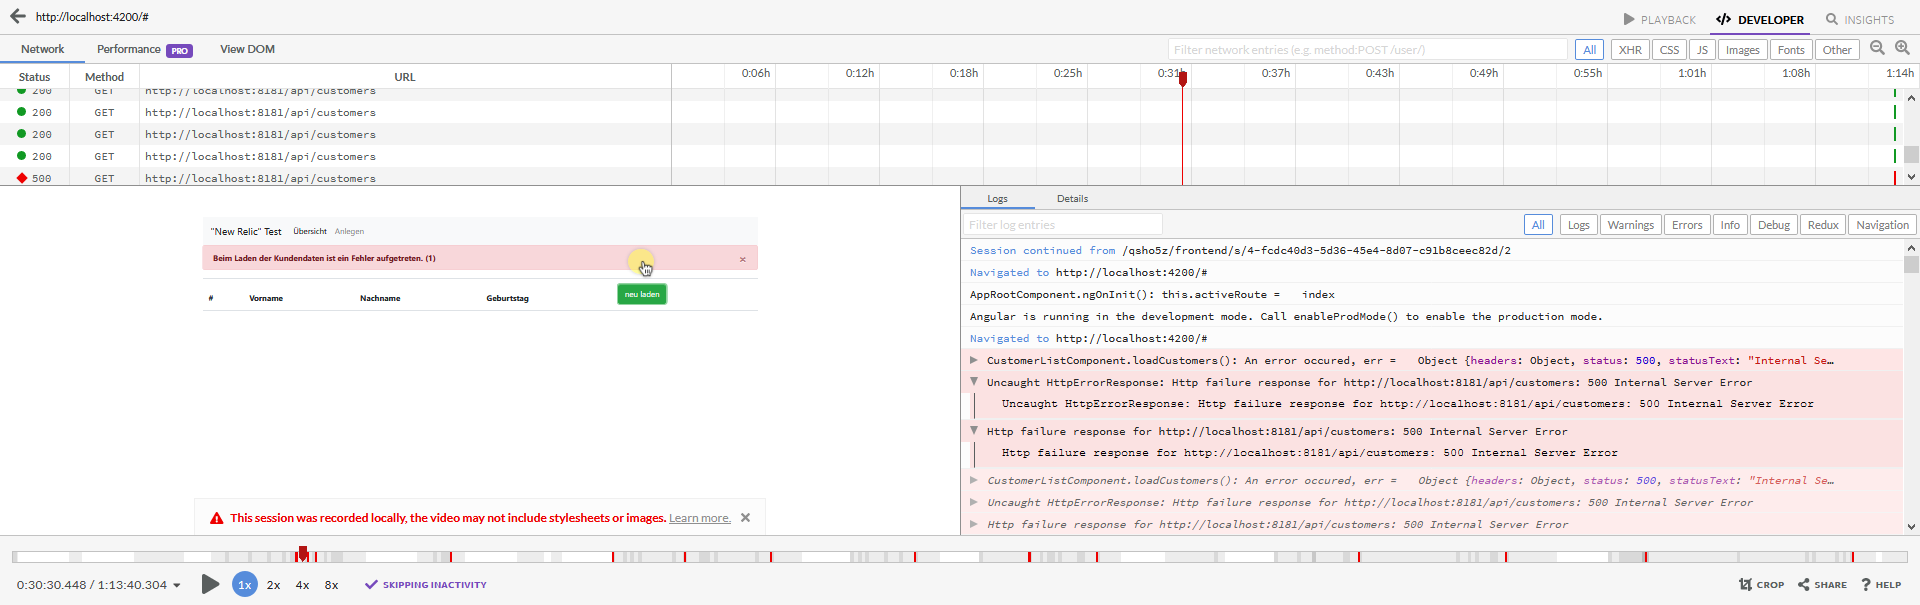
\includegraphics[width=\linewidth]{img/03_methoden/logrocket_session-replay-example.png}
	\caption{Beispiel eines Session-Replays bei LogRocket}
	\label{fig:logrocket-session-replay-example}
\end{figure}

\subsubsection{Splunk}

Splunk \cite{Splunk} ist ein Softwareprodukt und ein SaaS des gleichnamigen Unternehmens. Splunk fungiert als eine universelle Datensenke, z. B. für Metriken und Logdaten. Splunk bietet Funktionen diese Daten zu durchsuchen, überwachen, analysieren und visualisieren. Splunk wird klassisch für Log Management eingesetzt, kann aber auch Aspekte von APM, RUM und Error Monitoring erfüllen.

Splunks kostenlose Version der SaaS und der OnPremise-Lösung wurden evaluiert. Hierbei wurde zunächst festgestellt, dass das Daten senden vom Browserkontext zu Splunk nicht direkt möglich ist, da Splunk mit ablehnenden CORS-Headern antwortet. Hierfür wurde ein extra Dienst geschrieben, der die Daten vom Frontend annimmt und an Splunk weitersendet. Weiterhin konnten hierdurch Daten wie den User-Agent und die IP vom Client ermittelt und an die Datensätze angehangen werden.

An Splunk wurden über dieselbe Schnittstelle Log- und Errorinformationen gesendet. Hierbei konnte Splunk gut das Logmanagement erfüllen, denn Logeinträge ließen sich einfach filtern und auch zu Graphen aufbereiten. Weiterhin ist das Error Monitoring auch zufriedenstellend und enthält alle Daten, die auch bspw. bei Sentry vorhanden sind - hierbei fehlt jedoch ein Issue-Management, welches Sentry bereitstellt. Lediglich Tracing lässt sich nicht zufriedenstellend mit Splunk realisieren. Denn hier können lediglich die Daten konsumiert werden, aber eine verständliche Darstellung mittels Trace-Gantt-Diagrammen fehlt gänzlich. Hiermit lassen sich keine spezialisierten Tracing-Werkzeuge ersetzen.

\subsubsection{Honeycomb}

Honeycomb \cite{Honeycomb} ist ein SaaS der Hound Technology Inc. und verspricht die Speicherung vieler (Tracing-)Daten und darauf basierend effiziente Abfragen zu ermöglichen. Es ist hauptsächlich als Tracingdienst anzusehen, womit jedoch auch Aspekte des APM, RUM und Error Monitoring mit abgebildet werden können.

Honeycomb wurde mit der kostenlosen Version evaluiert. Honeycomb bietet sog. \enquote{Beelines} an, welche Werkzeuge zur automatischen Datenerfassung sind. Diese Beelines sind aber nur für Node.js, Go, Python, Java, Ruby und Rails verfügbar, aber nicht JavaScript im Browser. Deshalb wurden zur Evaluierung Werkzeuge von OpenTelemetry hinzugezogen und zusätzlich musste nur noch ein Exporter für Honeycomb geschrieben werden. Honeycomb wirkt komplett anders als New Relic und Dynatrace, denn es ist nicht ausgefertigt mit konkreten Graphen und Darstellungen, sondern bietet eine Oberfläche mit dem man auf Basis der Daten selber Abfragen, Graphen und andere Darstellungen selber erstellen kann. Auch ist es nicht mit Jaeger, welches gleich näher betrachtet wird, vergleichbar, denn es bietet deutlich mehr Möglichkeiten als striktes Tracing.

\subsubsection{Jaeger}

Jaeger wurde 2017 als ein Projekt der CNCF gestartet \cite{Jaeger}. Es ist ein System für verteiltes Tracing und bietet Funktionalitäten zur Datensammlung, -verarbeitung, -speicherung bis hin zur Visualisierung. Jaeger unterstützt und implementiert den Standard OpenTracing und erlaubt auch das Konsumieren von Zipkin Daten, einem Konkurrenzprodukt. Eine Unterstützung des OpenTelemetry Standards ist derzeit im Gange. Weiterhin kann Jaeger dazu benutzt werden, Metriken nach Prometheus \cite{Prometheus} zu exportieren, einem weiteren CNCF Projekt zur Speicherung und Visualisierung von Daten.

\begin{wrapfigure}[11]{r}{0.45\textwidth}
\centering
\vspace{-\baselineskip}
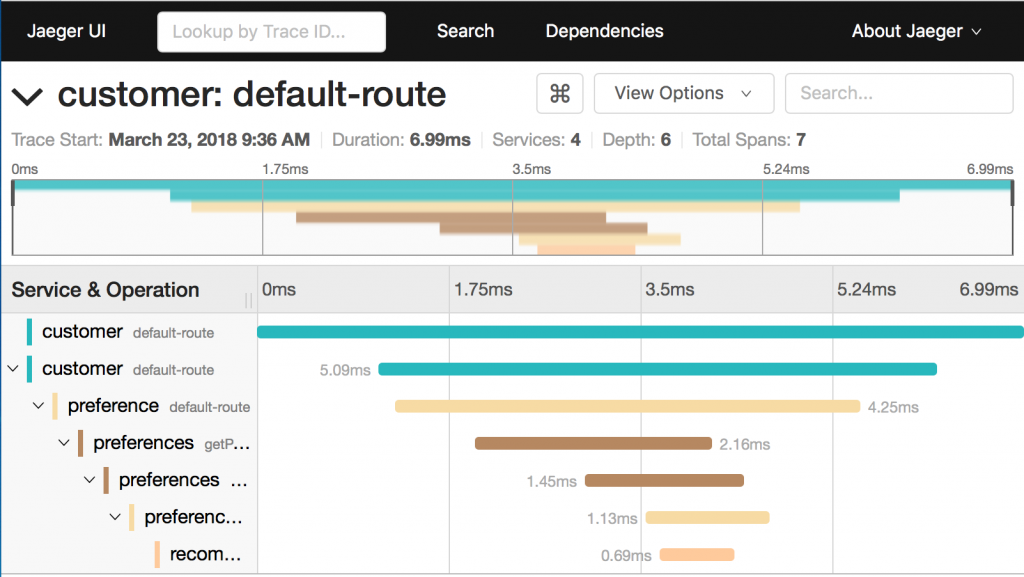
\includegraphics[width=\linewidth]{img/03_methoden/redhat_jaeger-ui_trace-detail-view.png}
\caption{Trace-Detailansicht. Quelle: Don Schenck \cite{JaegerIstioTracing}}
% von https://developers.redhat.com/blog/2018/04/03/istio-tracing-monitoring/
\label{fig:jaeger-ui_trace-detail-view}
\end{wrapfigure}

Jaeger wurde nicht aufgesetzt, sondern über einen Arbeitskollegen bei der Open Knowledge veranschaulicht und darauf basierend evaluiert. Wie zuvor bei Honeycomb beschrieben, beschränkt sich Jaeger auf Tracing, aber spezialisiert sich dafür auf dieses Gebiet und bietet eine gesamte Infrastruktur zur Tracespeicherung und -analyse. Die Traces sind als Gantt-Diagramme dargestellt, wie in \autoref{fig:jaeger-ui_trace-detail-view} zu sehen ist. Hierbei sind sowohl hierarchische als auch zeitliche Beziehungen visualisiert.

\begin{wrapfigure}[8]{r}{0.45\textwidth}
\centering
\vspace{-\baselineskip}
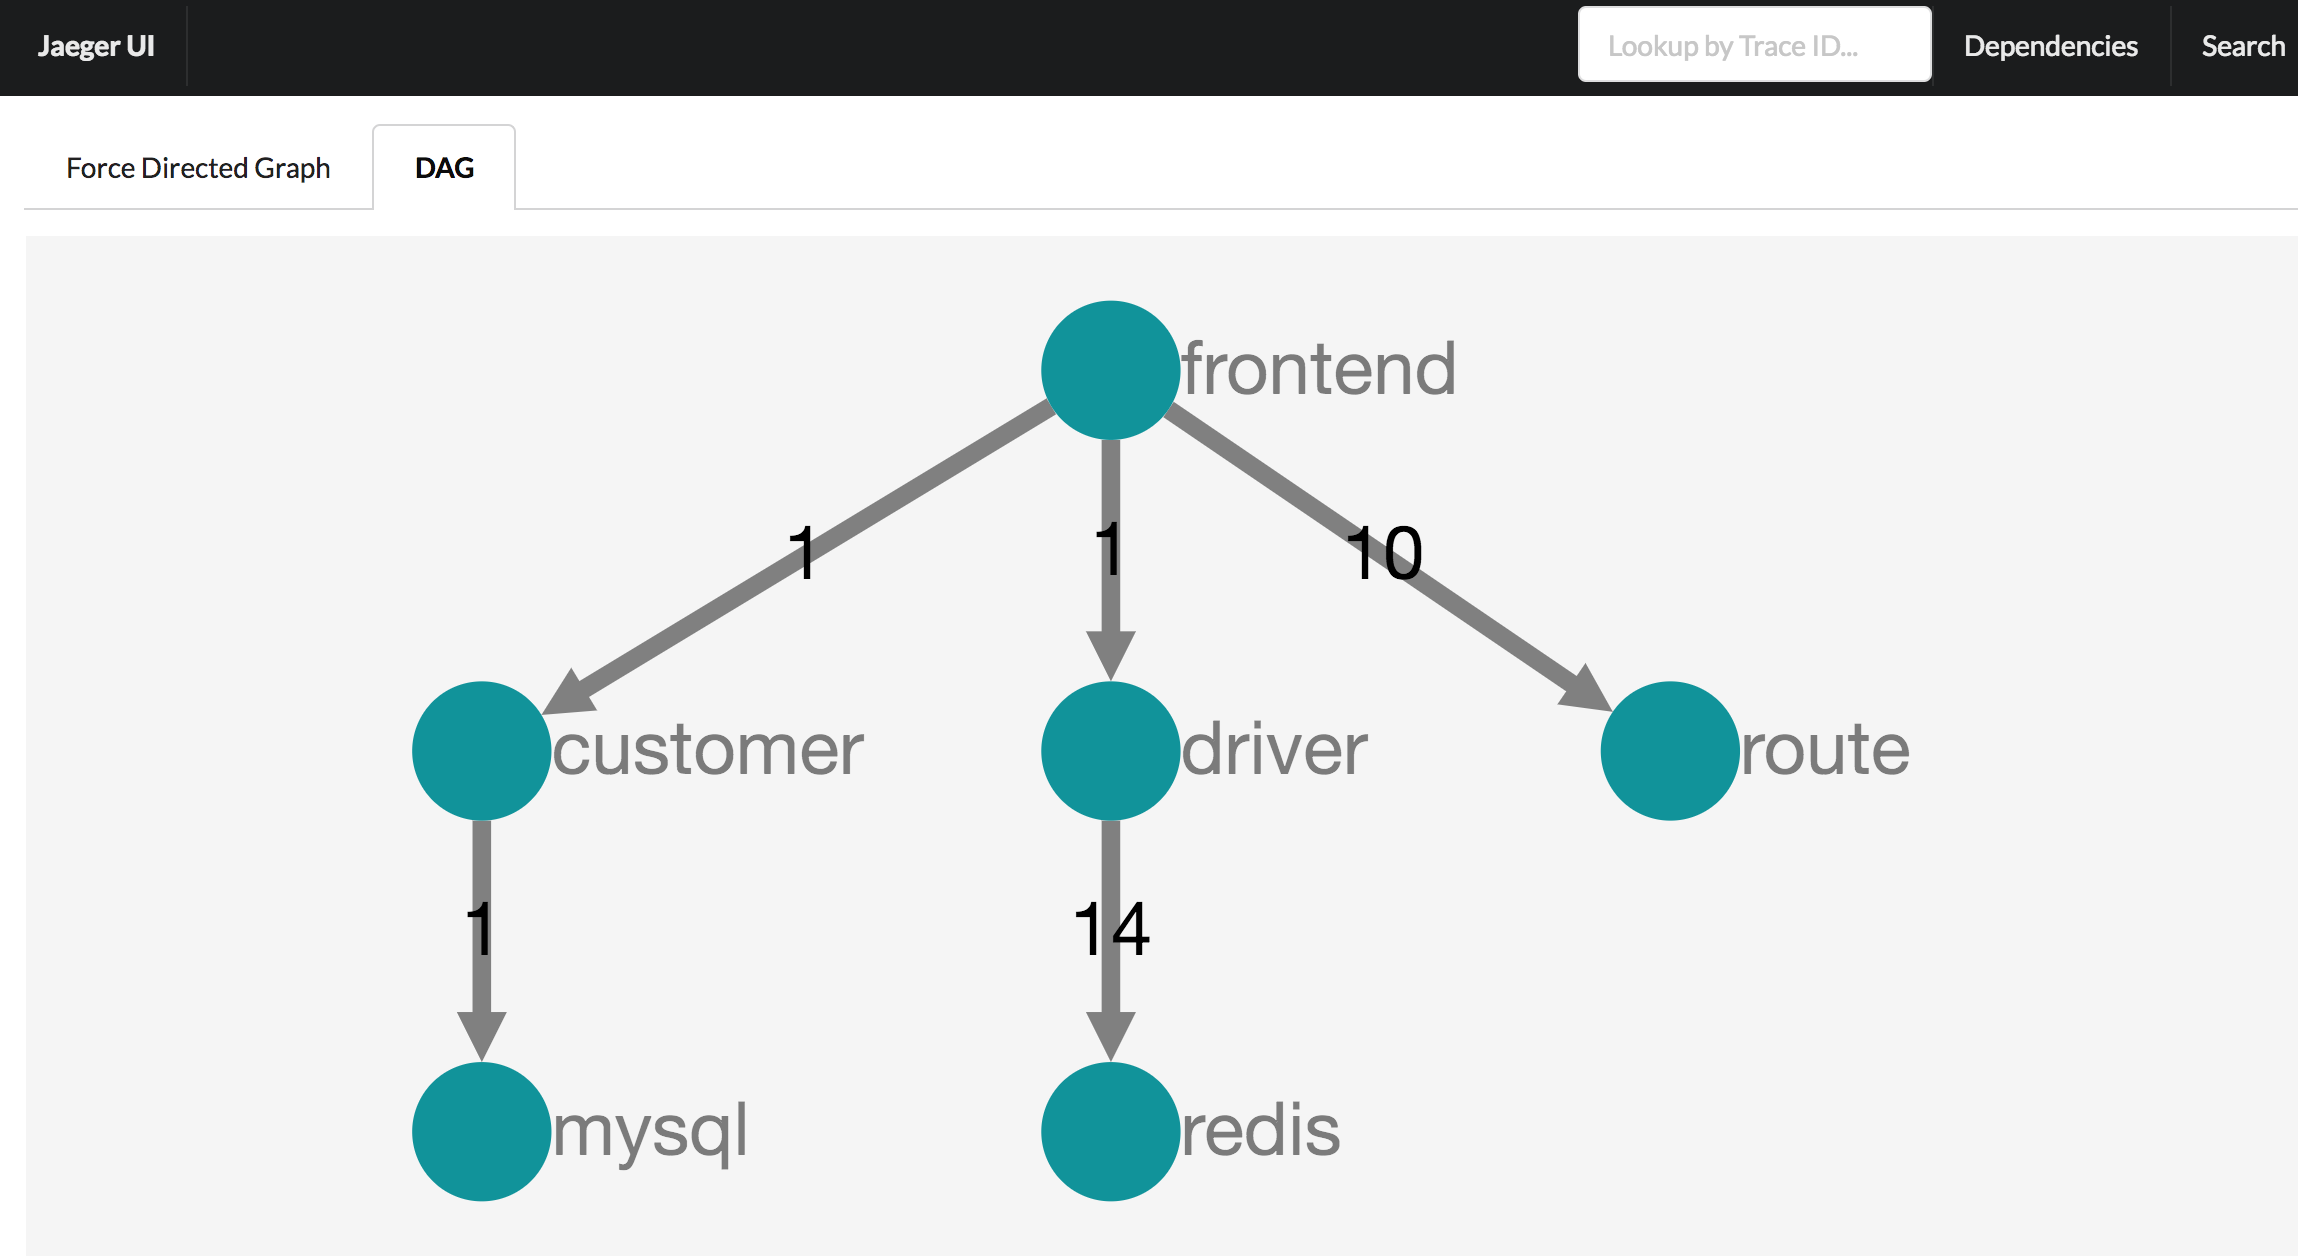
\includegraphics[width=\linewidth]{img/03_methoden/medium_jaeger-ui_dependency-graph.png}
\caption{Dienst-Abhängigkeits-Graph. Quelle: Yuri Shkuro \cite{JaegerTakeOpenTracingForARide}}
% von https://medium.com/opentracing/take-opentracing-for-a-hotrod-ride-f6e3141f7941
\label{fig:jaeger-ui_dependency-graph}
\end{wrapfigure}

Anhand der Traces generiert Jaeger zudem automatisch eine Architektur, indem die Beziehungen zwischen Diensten zu sehen ist. In \autoref{fig:jaeger-ui_dependency-graph} kann so eine Darstellung betrachtet werdenx, hierbei sieht mehrere Microservices und Datenbanken.

\subsubsection{Weiteres}
\label{sec:weitere-werkzeuge}

Bei der Recherche und Evaluierung wurden nicht alle auf dem Markt verfügbaren Werkzeuge und Technologien tiefergehend betrachtet. Deshalb werden weitere Funde, die nicht betrachtet wurden, hier kurz notiert:

\begin{itemize}
	\item APM \& RUM: AppDynamics, DataDog
	\item Error Monitoring: Airbrake, Instabug, Rollbar, Bugsnag, TrackJS
	\item Tracing oder Observability: Google Cloud Trace, Zipkin, Logz.io, Lightstep
\end{itemize}

Auch diese Auflistung stellt nicht die komplette Bandbreite an Werkzeugen und Technologien dar und die vorhergehende Betrachtung ist nicht als Empfehlung zu verstehen.

\subsection{Literatur}

In diesem Abschnitt sind die Ergebnisse aus der Literaturrecherche zusammengetragen: Verwandte Publikationen, die auf eine verbesserte Nachvollziehbarkeit abzielen.

%\begin{enumerate}
%	\item \textit{Gibt es hierzu Ansätze in der Literatur?}
%	\item \textit{Wie sehen diese aus, welchen Zweck erfüllen sie?}
%	\item \textit{Sind sie vergleichbar mit Ansätzen aus der Fachpraxis?}
%\end{enumerate}

\subsubsection{TraVista}

Ein erstes Werkzeug, welches in der Literatur identifiziert wurde, ist TraVista von Anand \etal \cite{TraVistaPaper}. Es basiert auf einem vorhergehenden Projekt von Anand, TraViz, welches nachgehend erläutert wird. TraVista beschäftigt sich mit dem Visualisieren von Tracedaten. Hierbei setzten sie auf den bestehenden Ansatz der Gantt-Diagramme auf, um Traces zu visualisieren. Die Gantt-Diagramme wurden jedoch um einige zusätzliche Informationen erweitert, wie in \autoref{fig:travista_extended-gantt} zu sehen ist.

\begin{wrapfigure}[8]{r}{0.3\textwidth}
\centering
\vspace{-1.5\baselineskip}
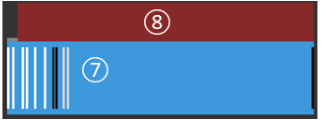
\includegraphics[width=\linewidth]{img/03_methoden/travista_extended-gantt_zoomed-in.png}
\caption{Zoom von \autoref{fig:travista_extended-gantt}, Abbildung aus \cite{TraVistaPaper}}
\label{fig:travista_extended-gantt_zoomed-in}
\end{wrapfigure}

Innerhalb eines Spans sind aufgetretene Events dargestellt, standardmäßig als weißer Balken oder bei selten auftretenden Events als schwarzer Balken (vgl. \circled{7} in \autoref{fig:travista_extended-gantt_zoomed-in}). Beziehungen \circled{6} zwischen den Spans werden visualisiert. Bei \circled{2} sind Histogramme zu sehen, die aus den gesammelten Metriken innerhalb der Traces, erstellt sind. Die Metrikwerte des aktuellen Trace sind blau hervorgehoben und erlauben hier auch eine visuelle Probe auf Ausreißer.

Es lässt sich abschließend sagen, dass TraVista eine vielversprechende Visualisierung bietet. Jedoch wurde ein eigenes simples Backend entwickelt, welches nur mit einer vergleichsweise geringen Datenmenge getestet wurde (22.286 Traces, 147.812 Spans). Die Autoren selbst sehen Probleme bei der Skalierung, aber nannten auch, dass sie TraVista weiterentwickeln wollen, um ein neues Backend zu entwickeln.

\begin{figure}[H]
	\centering
	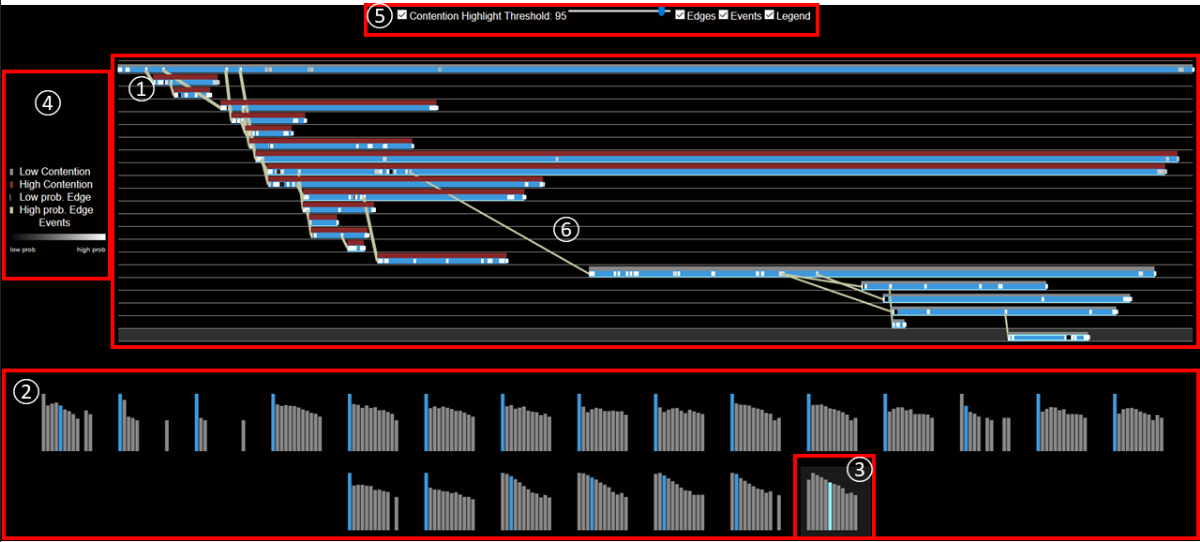
\includegraphics[width=0.815\linewidth]{img/03_methoden/travista_extended-gantt.png}
	\caption{TraVistas Gantt-Diagramm, Abbildung aus \cite{TraVistaPaper}}
	\label{fig:travista_extended-gantt}
\end{figure}

Vor der Arbeit an TraVista hat Vastaav Anand mit Matheus Stolet an einem weiteren Visualisierungstool für Traces gearbeitet: TraViz \cite{TraVizPaper}. Es ist auf GitHub veröffentlicht \url{https://github.com/vaastav/TraViz}. TraViz bildet das Grundgerüst für die spätere Arbeit an TraVista und ist zudem das Backend für TraVista. Im Genaueren bedeutet dies, dass TraVista ein neuer Visualisierungsansatz für das Backend von TraViz ist. Die meisten funktionalen Eigenschaften von TraVista lassen sich ebenso auf das Backend von TraViz zurückverfolgen.

Mit Joseph Wonsil hat Anand an einem weiteren Tool rund ums Tracing gearbeitet: Tracey \cite{TraceyPaper}. Es ist ebenso auf GitHub veröffentlicht \url{https://github.com/vaastav/Tracey}. Es beschäftigt sich mit der Aggregration von Tracingdaten, denn derzeitige Technologien beschäftigen sich hauptsächlich mit der Darstellung von einem einzelnen Trace. In diesem Bericht sind erneut Grundbausteine zu erkennen, die Anand wahrscheinlich bei TraVista anwenden konnte.

Sowohl TraViz (und TraVista) als auch Tracey werden jedoch seit Mai 2020 nicht mehr aktualisiert. Eine Nutzerschafft konnte auch nicht gefunden werden, da auf GitHub beide Projekte Null Mal favorisiert und Null Mal geklont wurden. Auch Issues oder Pull-Requests sind nicht vorhanden. Aufgrund dieser fehlenden Weiterentwicklung und den Skalierungsproblemen des Backends ist TraVista für diese Arbeit nicht von Relevanz. % Sollten sich jedoch in den nächsten Monaten und Jahren weitere Entwicklungen hier ergeben, könnte dieser Ansatz Früchte tragen.

\subsubsection{\enquote{Bedeutung von Telemetry für den SDLC}}

\nomenclature[Fachbegriff]{SDLC}{Software-Development-Life-Cycle}

Neben TraVista wurde die im 2. Quartal 2020 erstellte Bachelorarbeit von Michael Graf bei der Recherche gefunden \cite{MichaelGrafBA}. Grafs Arbeit handelt über die \enquote{Bedeutung von Telemetrie für den Software Development Cycle}. In der Arbeit beschäftigt er sich mit der Software-Telemetrie als solche, aber legt den aktuellen Stand am Projekt OpenTelemetry dar. OpenTelemetry erhält enorme Bedeutung in der Arbeit und wird von Grund auf erläutert, betrachtet und analysiert.

Die Arbeit beschäftigt sich zunächst mit SDLC und wie moderne Ansätze hierfür Aussehen. Speziell wird der DevOps Ansatz beschrieben, bei dem eine kontinuierliche Weiterentwicklung des Produktes im Vordergrund steht. Hierbei bewertet Graf die Fähigkeit von Observability-Ansätzen nach ihrem tatsächlichen Nutzen und ihrer Übertragbarkeit. Dies erfolgt, wie zuvor beschrieben, am Beispiel von OpenTelemetry. Evaluiert wird das Ganze durch das Aufsetzen von Jaeger mit einer Demoanwendung, durch das der Tracingaspekt von Observability realisiert wird.

Abschließend bewertet Graf OpenTelemetry positiv in den Punkten Interoperabilität, Plattformunabhängigkeit und Erweiterbarkeit. Jedoch mahnt er zudem, dass das Projekt noch jung ist und darauf basierend keine Prognosen über den Erfolg gemacht werden können. Graf sieht zudem Observabilitydaten als eine gute Möglichkeit, um die Qualitätssicherung und -verbesserung zu unterstützen.

Grafs Arbeit dient somit als Vorbereitung für einen Lösungsansatz mit OpenTelemetry, bietet aber selbst keine neuen Ansätze.

\subsubsection{Timelapse}

Burg \etal \cite{TimelapsePaper} entwickelten 2013 eine neue Software, die es erlaubt das Anwendungsverhalten von Webapplikationen aufzunehmen und wiederabzuspielen: \enquote{Timelapse}. Timelapse erlaubt es direkt im selben Browser Nutzersitzungen aufzunehmen und wieder abzuspielen, sodass die simulierten Aktionen im Browser geschehen. Dies bedeutet, dass Entwickler und Betreiber gleichzeitig den DOM inspizieren können und auch Breakpoints im JavaScript-Code verwenden können.

\begin{wrapfigure}[8]{r}{0.35\textwidth}
\centering
\vspace{-\baselineskip}
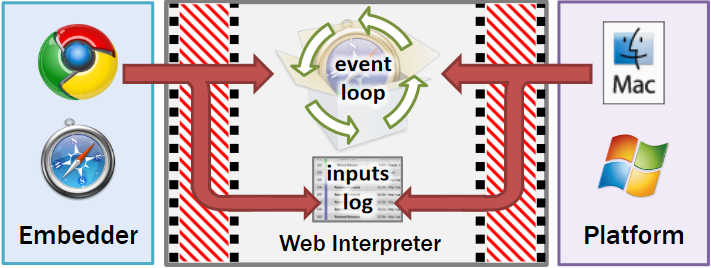
\includegraphics[width=\linewidth]{img/03_methoden/timelapse_figure5.png}
\caption{Mitschneiden von DOM-Events, Abb. aus \cite{TimelapsePaper}}
\label{fig:timelapse_figure5}
\end{wrapfigure}

Das Grundprinzip von Timelapse basiert darauf, dass die Browserumgebung gekapselt ist; sie lässt sich von außen nur über vordefinierte Schnittstellen ansprechen. Intern arbeit die Browserumgebung mit einem einzigen Thread indem eine Eventloop die Logik ausführt. Um nun die Aufnahme-/Abspielfunktionalität zu ermöglichen wird ein eigens entwickeltes Framework hinzugezogen, \enquote{Dolos}.

\begin{wrapfigure}[8]{r}{0.35\textwidth}
\centering
\vspace{-\baselineskip}
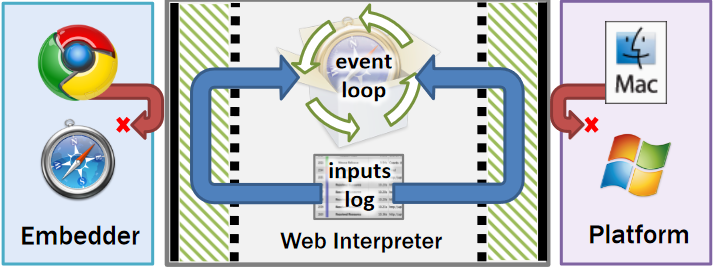
\includegraphics[width=\linewidth]{img/03_methoden/timelapse_figure6.png}
\caption{Abspielen von DOM-Events, Abb. aus \cite{TimelapsePaper}}
\label{fig:timelapse_figure6}
\end{wrapfigure}

Dolos schneidet interne DOM-Events sowie die Antworten von äußeren Schnittstellen mit (vgl. \autoref{fig:timelapse_figure5}). Beim Abspielen werden DOM-Events und äußere Aufrufe in derselben Reihenfolge der Eventloop übergeben (vgl. \autoref{fig:timelapse_figure6}). Hierbei wird die Eventloop von anderen Einflüssen abgeschottet, sodass eine exakte Rekonstruktion erfolgen kann. Bei der Rekonstruktion ist es von enormer Bedeutung nicht-deterministische Eingaben korrekt zu simulieren, also Tastatureingaben, Netzwerkanfragen aber auch interne Ressourcen wie Zufallswerte und die aktuelle Zeit.

Das Projekt ist sehr vielversprechend, besitzt jedoch einige Eigenschaften, die es mit der in dieser Arbeit angestrebten Lösung inkompatibel machen. Es benötigt eine tiefe Integration in den Browser, speziell wird eine gepatchte Version von WebKit benötigt. Dies ist einerseits aufwändig, aber in diesem Projektumfeld quasi unmöglich, da die Nutzer als vielzählig und unbekannt gelten und genau diese Nutzersitzungen sollten nachvollziehbar gemacht werden. Weiterhin unterstützt das Projekt nur den Safari und Google Chrome Browser, wahrscheinlich aber auch nicht die aktuellen, denn es wird seit mehr als 5 Jahren nicht mehr weiterentwickelt. Der Quellcode findet sich jedoch auf GitHub \url{https://github.com/burg/replay-staging/}. Insgesamt ist das Projekt somit ungeeignet für eine die angestrebte Lösung.

\subsubsection{FAME}

2018 arbeiteten Oriol \etal \cite{FamePaper} mit der Firma SEnerCon GmbH zusammen, um ein Framework zu Erstellen, welches Daten aus Nutzerfeedback und Monitoring kombiniert. SEnerCon wurde hinzugezogen, um das Framework zu evaluieren, die Entwicklung des Frameworks fand durch die Forscher selbst statt. Das Framework wurde FAME genannt und steht für \enquote{Feedback Acquisition and Monitoring Enabler}.

\begin{wrapfigure}[10]{r}{0.4\textwidth}
\centering
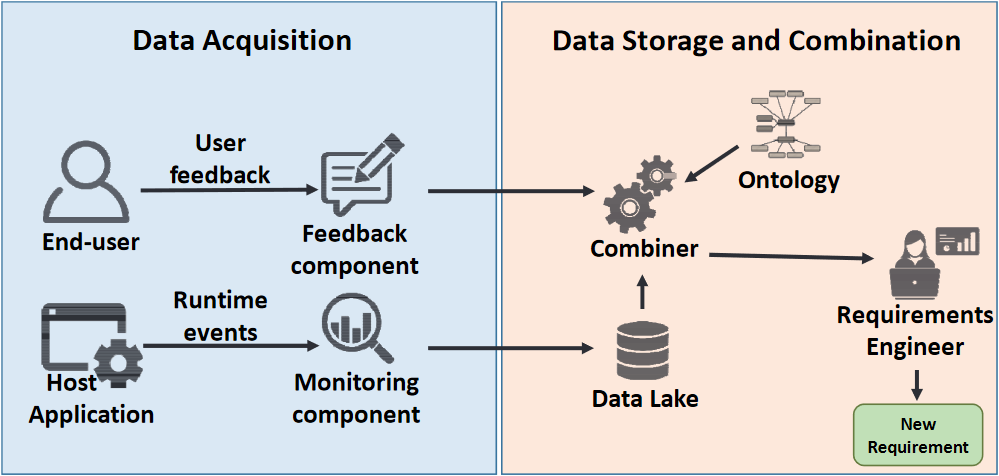
\includegraphics[width=\linewidth]{img/03_methoden/fame_overview.png}
\caption{Übersicht von FAME, Abb. aus \cite{FamePaper}}
\label{fig:fame_overview}
\end{wrapfigure}

Mit FAME wurde erforscht, ob die kombinierten Daten aus Nutzerfeedback und Monitoring dabei helfen können, um neue Anforderungen zu ergründen. Nach den Autoren ist dieser Ansatz neu, denn in der Literatur wurde zuvor hauptsächlich auf das Nutzerfeedback gesetzt um neue Anforderungen zu identifizieren. Dies ist aber von Problemen geplagt, wie bspw. dem Verständnis des Problems oder auch wie relevant dieses Problem für die gesamte Nutzerschaft ist. Mithilfe von der Addition von Monitoring sollen einige dieser Einschränkungen begegnet werden, indem bspw. Funktionsgebiete über Metriken abgebildet werden und wenn ein negatives Feedback eines Nutzers zu diesem Gebiet aufkommt, kann in der Metrik abgelesen werden, ob das Verhalten von anderen Nutzern sich geändert hat. Eine abstrakte Übersicht des FAME-Frameworks kann in \autoref{fig:fame_overview} betrachtet werden.

Das FAME-Framework definiert detailliert Komponenten, wie die Disziplin des Monitoring und der Feedbackeinholung gelöst werden können, und wie dies in einer möglichst modularen Infrastruktur umgesetzt werden kann. Für die Kombination der Monitoring- und Feedbackdaten werden zudem Mechanismen geschaffen, dass effiziente Queries diese beide zusammen verbunden ausgeben. Diese Ansätze wurden mit der SEnerCon GmbH in einem Workshop auf die Probe gestellt und konnten dem Requirements-Engineer dabei unterstützen, neue Anforderungen zu identifizieren und irrelevante Anforderungen auszuschließen. Es konnte ein Mehrwert für die SEnerCon GmbH identifiziert werden.

Das Framework FAME gehört zum größeren Projekt SUPERSEDE, welches von der EU gesponsert ist. Das Framework ist quelloffen unter GitHub verfügbar: \url{https://github.com/supersede-project/monitor_feedback}. Seit Ende 2018 wird es jedoch \textit{de facto} nicht mehr gewartet.

Das Projekt wird jedoch nicht bei der angestrebten Lösung verwendet. Zum Einen, weil das Ziel des Projektes nicht direkt auf Nachvollziehbarkeit von Nutzerinteraktionen und Anwendungsverhalten abzielt. Zu Anderem aber auch aufgrund der fehlenden Weiterentwicklung und Wartung. Dennoch sind die Erkenntnisse, dass eine Kombination aus unterschiedlichen Daten neue Sichtweisen ermöglicht, vielversprechend.

\subsubsection{The Kaiju Project}

Scrocca \etal \cite{TheKaijuProjectPaper} identifizierten 2020 eine Lücke im Gebiet der Observability, nämlich fehlt ein Werkzeug, welches die unterschiedlichen Datentypen Logs, Traces und Metriken kombiniert sammeln und aufbereiten kann und dies in quasi-Echtzeit. Aus diesem Grund wurde ein Konzept und ein Prototyp entwickelt, die darauf abzielen diese Lücke auszufüllen. Zunächst wird jedoch das Forschungsfeld und die Fachpraxis rund um die Observability aufgearbeitet. Hierbei definieren Scrocca \etal zwei Forschungsfragen, die es im Bericht zu beantworten gilt:

\begin{itemize}
	\item Wie können wir das Systemverhalten enthüllen?
	\item Wie können wir Sinn aus dem Systemverhalten gewinnen?
\end{itemize}

\begin{wrapfigure}[13]{r}{0.45\textwidth}
\centering
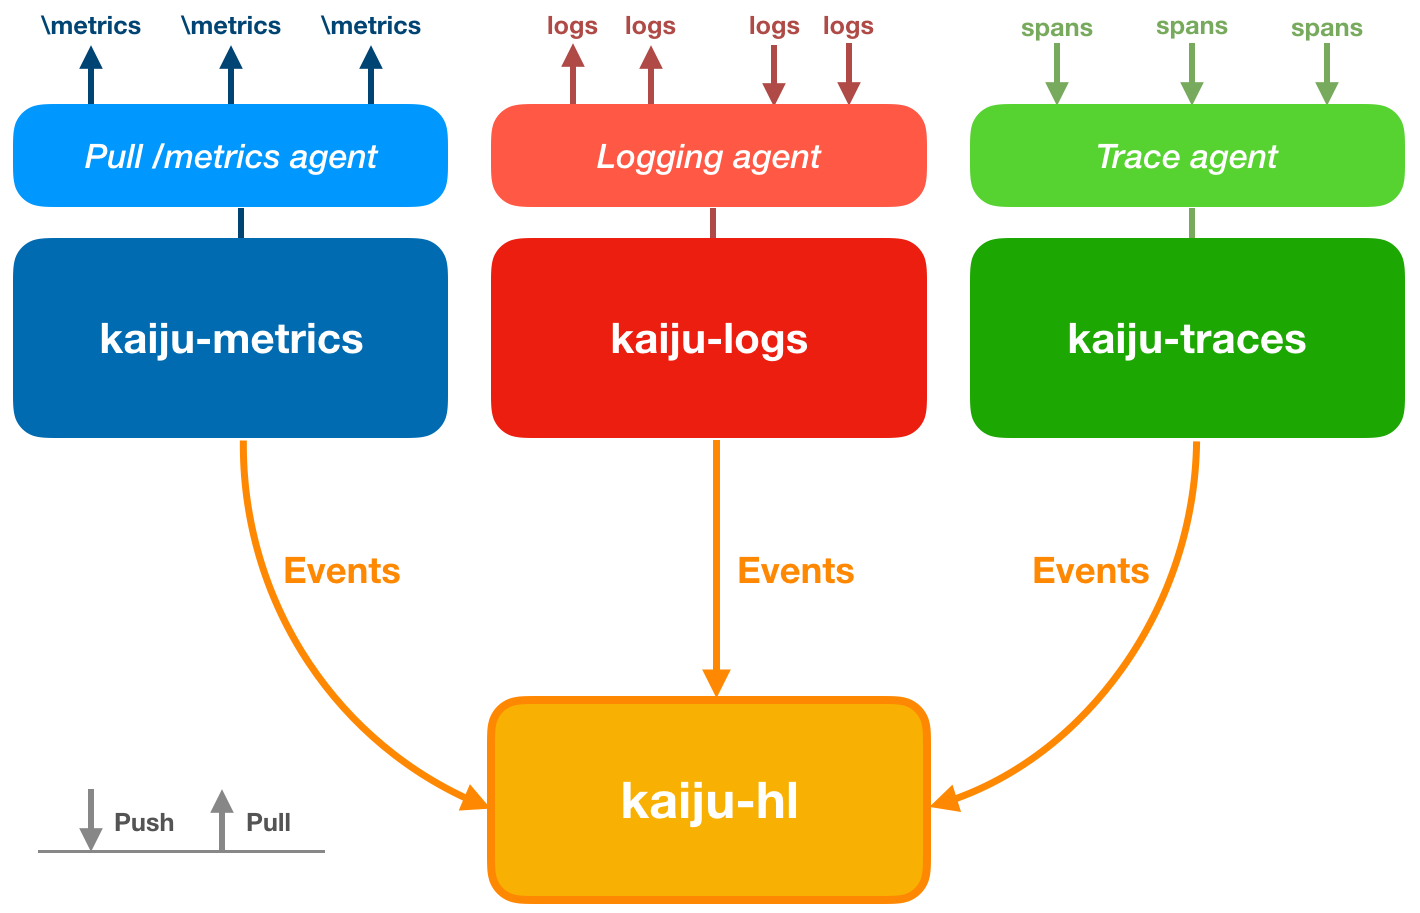
\includegraphics[width=\linewidth]{img/03_methoden/kaiju_architecture.png}
\caption{Kaiju Architektur, Abb. aus \cite{TheKaijuProjectPaper}}
\label{fig:kaiju_architecture}
\end{wrapfigure}

Um diese Forschungsfragen zu beantworten, wurde ein Konzept erstellt, wie die Datentypen Logs, Traces und Metriken zusammen erhoben und kombiniert analysiert werden können. Es basiert auf einer allgemeinen Datenverarbeitung mittels einem Event-Stream-Processor (ESP). Das Kernmodul stellt somit das \enquote{kaiju-hl} dar, welches in der Architektur in \autoref{fig:kaiju_architecture} zu betrachten ist. Das Hauptmodul besteht selber aus mehreren Subkomponenten, die spezielle analytische Aufgaben übernehmen. Der Prototyp wurde mit der quelloffenen ESP-Engine Esper \cite{Esper} umgesetzt.

\nomenclature[Fachbegriff]{ESP}{Event-Stream-Processor}

Aus den analysierten Daten erstellt Kaiju angereicherte und in der Struktur homogenisierte Daten, sogenannte High-Level-Events. Diese sind dann von weiteren Komponenten zu konsumieren. Diese praktische Weiterverarbeitung der gewonnenen Daten wurde jedoch nicht näher beleuchtet.

Nach der Entwicklung des Prototypen wurde aber in Zusammenarbeit mit der italienischen IT Dienstleistungsfirma SighUp dieser evaluiert. Es konnte festgestellt werden, dass abgeleitete High-Level Events, durch zuvor definierte Szenarien erstellt werden und Informationen beinhalten, die für die Problemfindung in diesen Szenarien hilfreich ist.

Der entwickelte Prototyp ist quelloffen unter \url{https://github.com/marioscrock/Kaiju} verfügbar. Dieser wurde aber seit Juli 2020, dem Zeitpunkt der Veröffentlichung des Papers, nicht mehr aktualisiert. Weiterhin lässt sich auch kein Folgeprojekt finden. Auch wenn Kaiju kein praktisches Werkzeug für die Lösung in dieser Arbeit darstellt, so wird ein gutes Bild über die technische Seite der Nachvollziehbarkeit vermittelt sowie wird zuvor der Forschungsstand erläutert.

\subsubsection{Fazit zur Literatur}

Wie auch in den verschiedenen beleuchteten Berichten und Arbeiten zu lesen ist, von denen drei in \textit{2020} veröffentlicht wurden, ist das Forschungsfeld der Nachvollziehbarkeit bzw. der Observability bisher nur spärlich untersucht worden. Es konnte ein Konsens identifiziert werden, dass dieses Forschungsfeld einen wichtigen Mehrwert darstellt, speziell bei komplexen Microservice-Architekturen.